\documentclass[10pt]{article}
\usepackage{float}
\usepackage[english]{babel}
\usepackage[utf8]{inputenc}
\usepackage[OT1]{fontenc}
\usepackage{amsfonts, amsmath, amsthm, amssymb}
\usepackage{graphicx}
\usepackage{listings}
\usepackage[margin=1in]{geometry}
\usepackage{xcolor}
\newcounter{countCode}
\lstnewenvironment{code} [1][caption=Ponme caption, label=default]{%
	\renewcommand*{\lstlistingname}{Listado} 
	\setcounter{lstlisting}{\value{countCode}} 
	\lstset{ %
	language=java,
	basicstyle=\ttfamily\footnotesize,       % the size of the fonts that are used for the code
	numbers=left,                   % where to put the line-numbers
	numberstyle=\sc,      % the size of the fonts that are used for the line-numbers
	stepnumber=1,                   % the step between two line-numbers. 
	numbersep=5pt,                 % how far the line-numbers are from the code
	numberstyle=\color{red!50!blue},
    	backgroundcolor=\color{lightgray!20},
	rulecolor=\color{blue},
	keywordstyle=\color{red}\bfseries,
	showspaces=false,               % show spaces adding particular underscores
	showstringspaces=false,         % underline spaces within strings
	showtabs=false,                 % show tabs within strings adding particular underscores
	frame=single,                   % adds a frame around the code
	framexleftmargin=0mm,
	numberblanklines=false,
	xleftmargin=5pt,
	breaklines=true,
	breakatwhitespace=true,
	breakautoindent=true,
	captionpos=t,
	texcl=true,
	tabsize=2,                      % sets default tabsize to 3 spaces
	extendedchars=true,
	inputencoding=utf8, 
	escapechar=\%,
	morekeywords={print, println, size, background, strokeWeight, fill, line, rect, ellipse, triangle, arc, save, PI, HALF_PI, QUARTER_PI, TAU, TWO_PI, width, height,},
	emph=[1]{print,println,}, emphstyle=[1]{\color{blue}}, % Mis palabras clave.
	emph=[2]{width,height,}, emphstyle=[2]{\bf\color{violet}}, % Mis palabras clave.
	emph=[3]{PI, HALF_PI, QUARTER_PI, TAU, TWO_PI}, emphstyle=[3]\color{orange!50!violet}, % Mis palabras clave.
	emph=[4]{line, rect, ellipse, triangle, arc,}, emphstyle=[4]\color{green!70!black}, % Mis palabras clave.
	%emph=[5]{size, background, strokeWeight, fill,}, emphstyle=[5]{\tt \color{red!30!blue}}, % Mis palabras clave.
	%emph={[2]sqrt,baset}, emphstyle={[2]\color{blue}}, % f(sqrt(2)), sqrt a nivel 2 se pondrá azul
	#1}}{\addtocounter{countCode}{1}}

%%%%%%%%%%%%%%%%%%%%%%%%%%%%%%%%%%%%%%%%%%%%%%%%
% Gaspare (Matteo) Staff
\theoremstyle{plain}
\newtheorem{thm}{Theorem} % reset theorem numbering for each chapter

\theoremstyle{definition}
\newtheorem{defn}[thm]{Definition} % definition numbers are dependent on theorem numbers
\usepackage{lmodern,textcomp}
\usepackage{amsmath}

\usepackage{array}
\newcolumntype{L}{>{\displaystyle}l}
\newenvironment{system}%
   {\setlength\arraycolsep{0pt}
    \left\lbrace \begin{array}{L}}%
   {\end{array} \right.}
   
\newcommand{\R}{\mathbb{R}}
\newcommand{\Z}{\mathbb{Z}}
\newcommand{\N}{\mathbb{N}}

\usepackage{caption}
\captionsetup[figure]{
    position=above,
}

    
\usepackage{pgfplots}
\usepackage{tikz}
\usepackage[utf8]{inputenc}

\usepackage{listings}
\usepackage{xcolor}

\definecolor{codegreen}{rgb}{0,0.6,0}
\definecolor{codegray}{rgb}{0.5,0.5,0.5}
\definecolor{codepurple}{rgb}{0.58,0,0.82}
\definecolor{backcolour}{rgb}{0.95,0.95,0.92}

\lstdefinestyle{mystyle}{
    backgroundcolor=\color{backcolour},   
    commentstyle=\color{codegreen},
    keywordstyle=\color{magenta},
    numberstyle=\tiny\color{codegray},
    stringstyle=\color{codepurple},
    basicstyle=\ttfamily\footnotesize,
    breakatwhitespace=false,         
    breaklines=true,                 
    captionpos=b,                    
    keepspaces=true,                 
    numbers=left,                    
    numbersep=5pt,                  
    showspaces=false,                
    showstringspaces=false,
    showtabs=false,                  
    tabsize=2
}

\lstset{style=mystyle}

%%%%%%%%%%%%%%%%%%%%%%%%%%%%%%%%%%%%%%%%%%%%%%%%

\title{\textbf{GTDMO - 2nd Assignment}}
\author{Group 6}
\pgfplotsset{compat = 1.17}
\begin{document}
\maketitle 

\section{Introduction to the Problem}

A survey is submitted to 15 customers of a restaurant asking them if 5 different aspects of the restaurant should be improved, namely
\begin{itemize}

\item  M1 = variety of starters
\item  M2 = variety of first dishes
\item  M3 = variety of cakes
\item  M4 = speed of service
\item  M5 = availability of parking
\end{itemize}
The collected data are stored in the file data6.csv. Higher grades correspond to an advice of bigger improvement, while low grades mean that the customer is satisfied of the present situation.

The collected data are represented in the following table
\begin{center}
 \begin{tabular}{|c c c c c c|} 
 \hline
  & M1 & M2 & M3 & M4 & M5 \\ [0.5ex] 
 \hline\hline
 1 & 0 & 0 & 1 & 13 & 7 \\ 
 \hline
2&	8&	8&	2&	0&	2 \\
\hline
3&	12&	7&	14	&0&	1\\
\hline
4&	0&	2&	1&	15&	11\\
\hline
5&	0&	0&	0&	13&	9\\
\hline
6&	1&	0&	1&	9&	10\\
\hline
7&	0&	0&	0&	14&	14\\
\hline
8&	9&	10&	10&	1&	1\\
\hline
9&	0&	1&	0&	11&	10\\
\hline
10&	0&	0&	0&	10&	6\\
\hline
11&	1&	0&	0&	13&	14\\
\hline
12&	0&	1&	0&	11&	11\\
\hline
13&	0&	0&	2&	7&	11\\
\hline
14&	13&	7&	8&	0&	1\\
\hline
15&	4&	12&	15&	0&	0\\[1ex] 
 \hline
\end{tabular}
\end{center}

\begin{enumerate}

\item Can you interpret the results in terms of ”concepts” behind the evaluation? 
\item Can you group and classify the customers with respect to their attention to such concepts?

\end{enumerate}



\section{Solution}
In order to answer the problem we can start running a preliminary analysis drawing an heatmap and looking for clusters in the columns of the dataset to better visualize the data: 
\begin{figure}[H]
	\centering
	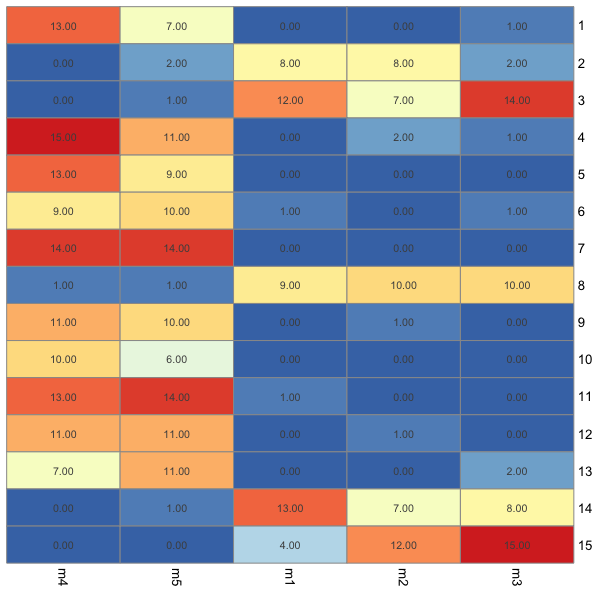
\includegraphics[scale=0.5]{figures/new01.png}
	\caption{M Matrix heatmap clustered by columns}
	\label{c1}
\end{figure}

As the clusterization suggests, we can easily notice that the customers seems to be split in 2 different groups:

\begin{itemize}

\item First group suggests strongly to improve the aspects regarding the speed of service and the availability of parking (M4 and M5).


\item Second group conveys that is the variety of dishes, that needs more improvement (M1, M2 and M3).

\end{itemize} 
Looking at some descriptive statistics we can highlight that
\begin{itemize}
    \item on average the suggestion of improvement is of 5 points (median) 
    \item the point that the clients have given more often is 0 (moda)
    \item the criteria 1 to 3 have lower necessity of improvement compared to the global average. 
    \item Instead, M4 and M5 are the aspects that are required of major improvements. 
\end{itemize}

As shown in the table below:
\newpage
\subsection{Part 1}
In order to answer the questions we begin by computing Singular Value Decomposition (SVD) of our matrix in \textit{R}. 
The SVD technique decomposes a matrix M of rank(n) into three components, three new matrices of rank(n):

\begin{equation}
    M = U\Sigma V^T
\end{equation}

where:

\begin{itemize}
    \item M is a nxd matrix 
    \item $\Sigma$ is a diagonal $r\times r$ matrix containing the singular values of M, of length min(n, p), in a decreasing order.
    \item U is an orthogonal $nxr$ matrix whose columns contain the left singular vectors of M, present if nu $>$ 0.
    \item $V^T$ is an orthogonal $rxd$ matrix whose columns contain the right singular vectors of M, present if nv $>$ 0. The original V matrix has, of course, dimension $dxr$.
\end{itemize}

The rank of our original Matrix $M$ is 5 as we can easily discover thanks to a few lines of code in \textit{R}. \\

We are initially interested just in $\Sigma$ among the three Matrices we decomposed $M$ in.
$\Sigma$ is a diagonal Matrix containing the Singular Values on its main diagonal and $0$ everywhere else. 
The Singular Values represent the weight of the "concepts" of the whole information of a Matrix but when these weights are small enough they can be ignored and cut off to both reduce the matrix size and to highlight the remaining ones.
From the preview obtained in the heatmap (Figure 1), we can already guess what the results of our $\Sigma$ will be.
\begin{equation}
\Sigma = 
\begin{bmatrix}
$50.045$ & $0$ & $0$ & $0$ & $0$ \\ 
$0$ & $36.444$ & $0$ & $0$ & $0$ \\ 
$0$ & $0$ & $9.879$ & $0$ & $0$ \\ 
$0$ & $0$ & $0$ & $6.600$ & $0$ \\ 
$0$ & $0$ & $0$ & $0$ & $6.254$ \\ 
\end{bmatrix}
\end{equation}

As a matter of fact, we can state that just the first $2$ values of them seem to account for more than 96\% of the information energy contained in our dataset as it can be better visualized in the figures below
\begin{equation}
\frac{\sum_{j=1}^2{\sigma_j^2}}{\sum_{j=1}^5{\sigma_j^2}} = \frac{50.04^2 + 36.44^2}{50.04^2 + 36.44^2 + 9.87^2 + 6.6^2 + 6.25^2}  = 0.96
\end{equation}

In Figure 2 it is possible to observe the graph rapidly tending to $0$ right after the second singular value, which is exactly what we seek in SVD.
\begin{figure}[H]
    \centering
    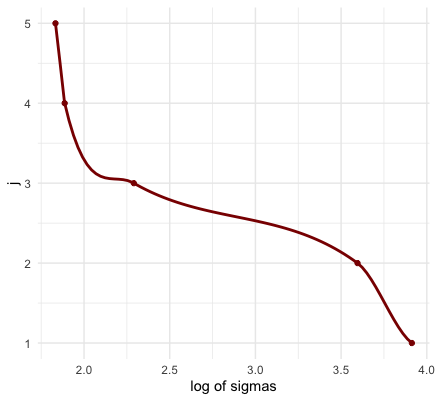
\includegraphics[scale=0.4]{figures/plo1.png}
    \caption{Plot of Log $\sigma_j$ against its own $j$}
    \label{fig:my_label2}
\end{figure}
From Figure 3 we can observe how the first singular value alone capture more than half of the total information energy while from the third on, every jump is always ticker than the previous one.
Note that in Figure $3$, with "Cumulative sum of sigmas over the sum of sigmas" it is actually meant \begin{equation}
\frac{\sum_{j=1}^r{\sigma_j}}{\sum_{j=1}^m{\sigma_j}}
\end{equation}
\begin{figure}[H]
    \centering
    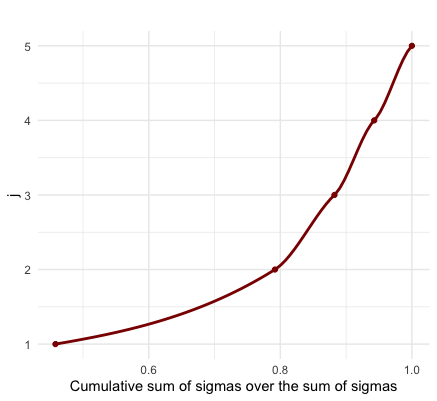
\includegraphics[scale=0.5]{figures/plot2.png}
    \caption{Ratio of the cumulative energy for every additional $\sigma$}
    \label{fig:my_label3}
\end{figure}

Truncating the Singular Values and their corresponding columns in U and rows in $V^T$  after 2 positions, we can obtain 3 new matrices $\tilde{U}$, $\tilde{\Sigma}$, $\tilde{V}$ of rank 2 which are the best approximation of M with a rank 2.

This can be formalized in the Eckart-Young Theorem which, in fact, states that the best absolute approximation to the Matrix M that has rank r is defined as:
\begin{equation}
    \underset{\tilde{M} s.t. rank(\tilde{M})=r}{\arg\min} ||M - \tilde{M}||_F   
\end{equation}
which it turns out to be exactly $\tilde{U}$$\tilde{\Sigma}$$\tilde{V^T}$.

The notation in the previous equation refers to the Frobenius norm, which is the square root of the summation of the squares of the differences between the individual matrix entries. It can be represented by the equation:

\begin{equation}
    ||A-B||_F = \sqrt{\sum_{ij}(A_{ij}-B_{ij})^2}
\end{equation}

This is how we are able to decompose a matrix into lower rank matrices without losing much of the relevant data.

\begin{equation}
M \approx \tilde{U} \tilde{\Sigma} \tilde{V}^T
\end{equation}

We can now conclude that keeping just the first 2 singular values allow us to retain more than 96\% of the informational energy of our data set but reducing the rank of M from 5 to 2. 
\newpage
What we are left with, then, are the equations (8) and (9). The $\tilde{U}$ matrix contains the left singular vectors representing the \textit{row to concept} similarity matrix while the $\tilde{V}$ matrix containing the right singular vectors represents the \textit{columns to concept} similarity matrix. $\tilde{\Sigma}$ contains of course the Singular Values, representing the weight of the \textit{concepts}.
\begin{equation}
\tilde{M} = \tilde{U} \tilde{\Sigma} \tilde{V}^T
\end{equation}
\begin{equation}
%\begin{align*}
\tilde{M} =
\begin{bmatrix}
$-0.286$ & $-0.040$ \\ 
$-0.054$ & $0.267$ \\ 
$-0.066$ & $0.524$ \\ 
$-0.371$ & $-0.025$ \\ 
$-0.310$ & $-0.061$ \\ 
$-0.268$ & $-0.016$ \\ 
$-0.391$ & $-0.073$ \\ 
$-0.074$ & $0.449$ \\ 
$-0.296$ & $-0.041$ \\ 
$-0.227$ & $-0.045$ \\ 
$-0.378$ & $-0.055$ \\ 
$-0.309$ & $-0.043$ \\ 
$-0.252$ & $-0.009$ \\ 
$-0.056$ & $0.434$ \\ 
$-0.051$ & $0.494$ \\ 
\end{bmatrix} 
\begin{bmatrix}
$50.045$ & $0$ \\ 
$0$ & $36.444$ \\ 
\end{bmatrix}%
\begin{bmatrix}
$-0.069$ & $-0.080$ & $-0.088$ & $-0.737$ & $-0.662$ \\ 
$0.549$ & $0.525$ & $0.635$ & $-0.126$ & $-0.065$ \\ 
\end{bmatrix}
%\end{align*}
\end{equation}

Now we can finally interpret the results in terms of "concepts" dividing the 5 initial questions of our survey in 2 main groups:

\begin{enumerate}
\item the first group, i.e. the group whose concern is greatest, and therefore the one the restaurant should be most aware of, is mainly interested with what can be conceptualized as \textit{services quality}:
\begin{itemize}
\item M4 = speed of the service

\item M5 = parking availability
\end{itemize}

\item The second group is composed by the first 3 aspects, respectively:
\begin{itemize}
\item M1 = variety of starters 
\item M2 = variety of first dishes 
\item M3 = variety of cakes 
\end{itemize}
These 3 aspects seems instead to have a slightly minor weight in customer's concerns. They can be summarized in the concept of \textit{courses variety }.
\end{enumerate}
\newpage
\subsection{Part 2}
The second question can be addressed just by looking at the $\tilde{U}$ matrix that, as stated above, proposes the strength of the similarity between customers and the concepts.

\begin{equation}
\tilde{U} =\begin{bmatrix}
$-0.286$ & $-0.040$ \\ 
$-0.054$ & $0.267$ \\ 
$-0.066$ & $0.524$ \\ 
$-0.371$ & $-0.025$ \\ 
$-0.310$ & $-0.061$ \\ 
$-0.268$ & $-0.016$ \\ 
$-0.391$ & $-0.073$ \\ 
$-0.074$ & $0.449$ \\ 
$-0.296$ & $-0.041$ \\ 
$-0.227$ & $-0.045$ \\ 
$-0.378$ & $-0.055$ \\ 
$-0.309$ & $-0.043$ \\ 
$-0.252$ & $-0.009$ \\ 
$-0.056$ & $0.434$ \\ 
$-0.051$ & $0.494$ \\ 
\end{bmatrix} 
\end{equation}

We can further analyze this classification by computing the  \textit{"similarity to the concepts" score} of every single user and comparing them together.
If we represent the customer with her/his new surveys preferences vector $\Vec{m}$, we can compute a score vector as

\begin{equation}
\Vec{s}_j = \Vec{u}_j\tilde{V}
\end{equation}

where $\Vec{u}_j$ is the vector related to customer $j$ and $V$ is the matrix of our SVD mapping the aspects of the survey to the concepts. Note that we could do this for every new customer and check for their affiliation to the concepts. 
If we want this for every customer, we can simply multiply

\begin{equation}
S = \tilde{M}\tilde{V}
\end{equation}

obtaining

 \begin{figure}[H]
	\centering
	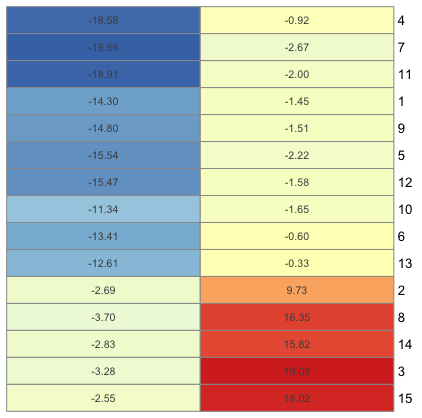
\includegraphics[scale=0.5]{figures/new02.png}
	\label{fig4}
\end{figure}

Where the $j-th$ row represent the score vector of user $j$.
\newpage
If we assign a number to every customer we can easily classify them in 2 groups:
\begin{enumerate}
	\item Users $\{1,4,5,6,7,9,10,11,12,13\}$ are heavy related to the concept represented by the first singular value, therefore are more concerned with improving \textit{services quality} of the restaurant.
	\item Users $\{2,3,8,14,15\}$ are instead highly related to the concept represented by the second singular value 	and they are indeed more interested in improving the \textit{courses variety} of the restaurant.
\end{enumerate}
\newpage
\subsection{Appendix}
For the sake of Reproducibility Research, here I attach the full commented R code used to obtain all Figures, Tables, equations and results.
\\
\lstinputlisting[language = R]{figures/Assign_2.R}
\end{document}
